\documentclass[10pt]{article}
\setlength{\parskip}{0.25\baselineskip}
\usepackage[margin=1in]{geometry} 
\usepackage{amsmath,amsthm,amssymb, graphicx, multicol, array}
\usepackage[font=small,labelfont=bf]{caption}

\newcommand{\supp}{{\text{supp}}} 
\newcommand{\bv}{{\text{BV}}}
\newcommand{\ac}{{\text{AC}}}

\newenvironment{problem}[2][]{\begin{trivlist}
\item[\hskip \labelsep {\bfseries #1}\hskip \labelsep {\bfseries #2.}]}{\end{trivlist}}

\begin{document}
 
\title{Midterm \#1}
\author{Eric Tao\\
Math 237: Midterm \#1}
\maketitle

\begin*{}
The Tufts University statement on academic integrity holds that: “Academic integrity is the joint responsibility of faculty, students, and staff. Each member of the community is responsible for integrity in their own behavior and for contributing to an overall environment of integrity at the university.”  I accept this responsibility, affirm that I am an honest person who can be trusted with to do the right thing, and certify that the work I will do on this exam is mine alone. I pledge that I have used only the reference sources I have cited in my answers.

Digital Signature: Eric Tao
\end*{}
\pagebreak

\begin{problem}{Question 1}

Let $(X, \rho)$ be a compact metric space, and $f: X \to X$ a function such that:

$$ \rho(f(x), f(y)) < \rho(x,y) $$

for all $x \not = y$.

Define $g: X \to \mathbb{R}$ via $g: x \mapsto \rho(x, f(x))$.

1.1)

Prove that $g$ is Lipschitz, and that $g$ has a minimum value, achieved at a point $x_0 \in X$. Conclude that there exists $x \in X$ such that $g(x) = 0$.

1.2)

Show that $f$ has a unique fixed point $x_0$.

1.3)

Show that the assumption that $X$ is compact may not be omitted.

\end{problem}
\begin{proof}[Solution]

1.1)

Fix some $x \in X$, and let $y \in X$ be arbitrary. By the triangle inequality, we see that:

$$ \begin{cases} \rho(x, f(x)) \leq & \rho(x,y) + \rho (y, f(x)) \\ \rho(y, f(x)) \leq & \rho(y, f(y)) + \rho(f(x), f(y)) \end{cases}$$

Combining these two equations with the property of $f$ by hypothesis, we see that:

$$ \rho(x, f(x)) - \rho(y, f(y)) \leq \rho(x,y) + \rho(f(x), f(y)) < 2 \rho(x,y) $$

However, we notice that we may run the same computation in the triangle inequality, switching the labels of $x, y$, as $\rho(x,y) = \rho(y,x)$. Thus, we can conclude then that

$$ | \rho(x, f(x)) - \rho(y, f(y))| < 2 \rho(x,y)$$

and therefore, since the left side is exactly $d(g(x), g(y))$ with the metric of the real line, we may conclude that $g$ is Lipschitz with Lipschitz constant at most 2.

Now, since $g$ is Lipschitz continuous, it is continuous. Hence, since $X$ is compact, $g$ achieves its extremas. Hence, we may find $x_0 \in X$ such that $g$ achieves its minimum value.

Suppose that $g(x_0) > 0$. Then, of course, we would have that $g(x_0) = \rho(x_0, f(x_0)) > 0$ and hence, $x_0 \not = f(x_0)$. Then, we can consider $g(f(x_0))$. We have that:

$$ g(f(x_0)) = \rho(f(x_0), f(f(x_0))) < \rho(x_0, f(x_0)) = g(x_0)$$

But, this is a contradiction, as we assumed that $g$ attained a minimum at $x_0$. Hence, $g(x_0) = 0$.

1.2)

From 1.1, we've shown that there exists $x_0 \in X$ such that $g(x_0) = 0$. Evidently then:

$$ g(x_0) = 0 \implies \rho(x_0, f(x_0)) = 0 \implies f(x_0) = x_0$$

Furthermore, this point must be unique, as suppose $f(x_1)= x_1$ as well. Assuming that $x_0 \not = x_1$, we have that:

$$ \rho(x_0, x_1) = \rho(f(x_0), f(x_1)) < \rho(x_0, x_1) $$

which is absurd. Hence, $x_0 = x_1$. 

1.3)

Here are some examples to show that we need $X$ to be compact. Consider $X = \mathbb{Z}$, equipped with the standard metric $\rho(x,y) = | x - y | $. Of course, this is not compact, as the sequence $\{ n \}_{n=1}^\infty$ cannot admit any convergent subsequence. If we take $f(x) = \operatorname{round}(x/2)$, where the round function rounds to the integer closer to $0$, then of course, we have that $\rho(f(x), f(y)) < \rho(x,y)$ for $x \not = y$, as it contracts all distances by at least 1/2. On the other hand, it has multiple fixed points, $-1, 0, 1$.

Another example is to take the open interval $(0,1)$, equipped with the standard metric $\rho(x,y)$, and consider the function $f(x) = x/2$. Evidently, in the same fashion, we still have that $\rho(f(x), f(y)) = | x/2 - y/2 | = 1/2 | x- y | = 1/2 \rho(x,y) < \rho(x,y)$. However, $g$ does not attain a minimum and $f$ does not have a fixed point.

We can see $g$ does not have a minimum as for any $\epsilon > 0$, we may choose $N \geq 1$ such that $1/N < \epsilon$. Then, $g(1/N) = \rho(1/N, f(1/N)) = | 1/N - 1/2N | = 1/2N < 1/N < \epsilon$. Hence, $g(x)$ can be arbitrarily small. However, we can see that for $x = 1/2x$, this is satisfied only at $x = 0$, outside of $(0,1)$. Hence, there is no $x$ such that $g(x) = 0$ on $(0,1)$, and no fixed point of $f$ on $(0,1)$.

\end{proof}
\pagebreak
\begin{problem}{Question 2}

Let $X, Y$ be Banach spaces. Let $T \in L(X,Y)$. Show that $T$ is surjective if and only if $\operatorname{range}(T)$ is not meager in $Y$.

\end{problem}

\begin{proof}[Solution]

One direction is trivial. Suppose $T$ is surjective. Then, $Y = \operatorname{range}(T)$. But, by the Baire Category Theorem (2.21, Heil), $Y$ is nonmeager in $Y$, and we are done.

Now, suppose $\operatorname{range}(T)$ is not meager. Consider open balls in $X$ centered on the origin, $B_n^X(0) = \{ x \in X : \Vert x \Vert < n \}$, where we use the superscript to remind ourselves this is in $X$. Clearly, $X = \cup_{n=1}^\infty B_n^X(0)$. Therefore, we have that the range of $T$ can be expressed as:

$$ \operatorname{range}(T) = \cup_{n=1}^\infty T(B_n^X(0)) $$

Since $T$ is non-meager, there exists an $m$ such that the closure $\overline{T(B_m^X(0)}$ contains an open ball, as its complement is not dense. We can consider the operator $mT$, and the closure $\overline{mT(B_1^X(0))}$ contains an open ball in $Y$, as $T(B_m^X(0) = mT(B_1^X(0))$ by linearity. Then, by Lemma 2.26 in Heil, we have that $mT(B_1^X(0))$ contains an open ball $B_r^Y(0)$ for some $r > 0$. Again, by linearity then, we have that $T(B_m^X(0)$ contains an open ball $B_{r/m}^Y(0)$.

So now, let $y \in Y$. In particular, consider $\frac{y}{\Vert y \Vert} * \frac{r}{2m}$. Evidently, the norm of this vector is $r/2m$, and hence is contained within $B_{r/m}^Y(0)$. Thus, there exists an $x \in X$ such that $T(x) = \frac{y}{\Vert y \Vert} * \frac{r}{2m}$. By linearity then, we have that:

$$T\left( \frac{2mx \Vert y \Vert}{r} \right) = \frac{2m\Vert y \Vert}{r} T(x) =  \frac{2m\Vert y \Vert}{r} \frac{y}{\Vert y \Vert}  \frac{r}{2m} = y$$

Hence, $Y \subseteq \operatorname{range}(T)$, and therefore, $Y = \operatorname{range}(T)$. Thus, $T$ is surjective. 

\end{proof}
\pagebreak
\begin{problem}{Question 3}

Let $C_b(\mathbb{R})$ be the space of bounded, continuous, real-valued functions. Let $C^1_b(\mathbb{R})$ be the space of functions such that $f, f' \in C_b(\mathbb{R})$. Equip both of these spaces with the uniform norm.

3.1)

Show that $C_b$ is complete, and that $C^1_b$ is not complete.

3.2)

Show that the differentiation operator $D: C^1_b(\mathbb{R}) \to C_b(\mathbb{R})$ that sends $D: f \mapsto f'$ is unbounded, but has a closed graph.

\end{problem}

\begin{proof}[Solution]

3.1)

First, consider the family of functions $f_n(x) = 2^{-n} \cos(7^n \pi x)$ for $n \geq 1$, and consider $g_m(x) = \sum_{n=1}^m f_n(x)$.

We have that the sequence of $\{ g_m \}$ is uniformly Cauchy, as if we let $\epsilon > 0$, we may choose $N$ such that $2^{-N+1} < \epsilon$, and then for $m, m' > N$ (WLOG, suppose $m > m'$), we have that:

$$ | g_m(x) - g_{m'}(x) | = | \sum_{n=1}^m f_n(x) - \sum_{n=1}^{m'} f_n(x)| = | \sum_{n=m}^{m'} f_n(x)| \leq | \sum_{n=N}^\infty f_n(x) |  \leq \sum_{n=N}^\infty |f_n(x)|  \leq \sum_{n=N}^\infty 2^{-N} = 2^{-N+1}$$

Since this is independent of the point $x$, this is uniformly Cauchy. Since each $g_m$ is continuous, being the finite sum of continuous functions, and the convergence is uniform, the pointwise limit $g(x) = \lim_{m \to \infty}g_m(x)$ is a continuous function. Moreover, we can see easily that $g$ is bounded, as we can see that each of the partial sums are bounded above by $\sum_{n=1}^\infty 2^{-n} = 2$. However, this is a Weierstrauss function, famously known for being differentiable nowhere. Since we have demonstrated a sequence of functions in $C^1_b$, convergent under the uniform norm to a function not in $C^1_b$, we may conclude that $C^1_b$ is not complete.

On the other hand, let $\{ f_n \}_{n=1}^\infty \subseteq C_b$, with $\sum_{n=1}^\infty \Vert f_n \Vert_u < \infty$. Consider $f = \sum_{n=1}^\infty f_n$, and we will show that $f$ is both bounded, and the uniform limit of the partial sums.

Evidently, $f$ is bounded, as we can look at the partial sums $ \sum_{n=1}^N f_n$. We have that $\Vert \sum_{n=1}^N f_n \Vert_u \leq \sum_{n=1}^N \Vert f_n \Vert_u  < \sum_{n=1}^\infty \Vert f_n \Vert_u < \infty$, where the first inequality comes from the triangle inequality, and the second is simply our hypothesis of being absolutely convergent. Since this bound holds for all $N > 0$, it must hold in the limit as well. Hence, $\Vert f \Vert_u < \sum_{n=1}^\infty \Vert f_n \Vert_u < \infty$.

Now, we wish to show that $\sum_{n=1}^N f_n \to f$ uniformly. Since $\sum_{n=1}^\infty \Vert f_n \Vert_u < \infty$, for $\epsilon > 0$, we may find a $M > 0$ such that for all $m > M$,  $\sum_{n=M}^\infty \Vert f_n \Vert_u < \epsilon$. Now, let $m > M$, and consider $\Vert f - \sum_{n=1}^m f_n \Vert_u$. We see that:

$$ \Vert f - \sum_{n=1}^m f_n \Vert_u = \Vert \sum_{n=m+1}^\infty f_n \Vert_u$$

Now, due to the positivitiy of the norm, since we have for each finite sum: $\Vert \sum_{n=m+1}^p f_n \Vert_u \leq \sum_{n=m+1}^p \Vert f_n \Vert_u \leq \sum_{n=m+1}^\infty \Vert f_n \Vert_u$, we may conclude that this holds in the limit as well.

Hence, we have that:

$$ \Vert \sum_{n=m+1}^\infty f_n \Vert_u \leq \sum_{n=m+1}^\infty \Vert f_n \Vert_u < \epsilon $$

Thus, $f_n \to f$ uniformly, and hence, $f$ is continuous. Therefore, $f \in C_b$, as desired, and $f_n \to f$ under the norm. Since the choice of absolutely convergent sequence was arbitrary, by 5.1 in Folland, since every absolutely convergent sequence converges, $C_b$ must be complete.

3.2)

Evidently, $D$ is unbounded. For example, take the family of functions $f_k = \sin(kx)$, for $k \in \mathbb{N}$. Clearly, this is a continuous function, bounded above by 1, and so $\Vert f_k \Vert_u = 1$. Furthermore, its derivative is $k \cos(kx)$, continuous, and for each $k$, bounded above by $k$. However, $ \Vert D(f_k) \Vert_u = \Vert k \cos (kx) \Vert_u = k$. Since we may choose $k$ arbitrarily large without affecting the norm of $f_k$, $D$ is unbounded.

Now, suppose that we have $f_n \to f \in C^1_b$, and $Df_n = f'_n \to g \in C^1$, uniformly in both cases. Fix an arbitrary point $a \in \mathbb{R}$, and consider, for $x > a$, the closed interval $[a,x]$. Since we have that $f'_n \to g$ uniformly, evidently, $\Vert f'_n \Vert_u$ is bounded. Then, we can take $\sup_{n} \Vert f'_n \Vert_u < \infty$ as an upper bound for all $|f'_n(y)|, y \in [a,x]$. Of course also, if $f'_n \to g$ uniformly, it does so pointwise as well. Therefore, by the Lesbesgue Dominated Convergence Theorem, we have that:

$$ \lim_{n \to \infty} \int_a^x f'_n(y) dy = \int_a^x g(y) dy $$

However, we know that $f_n$ is differentiable on $[a,x]$, and $f'_n$, its derivative is continuous. Thus, we may transform the left hand side via the Fundamental Theorem of Calculus to obtain:

$$ \lim_{n \to \infty} f_n(x) - f_n(a) = \int_a^x g(y) dy$$

Now, since $f_n \to f$ uniformly, it does so pointwise as well, so we have that:

$$ f(x)  - f(a) = \int_a^x g(y) dy$$

and finally, we can apply $D$ to both sides of this equation, and since $g$ is continuous, we can apply the other statement of the FTC to obtain:

$$ D(f(x) - f(a)) = D\left(\int_a^x g(y) dy \right) \implies D(f)(x) = g(x) $$

Since the choice of $a$ were arbitrary, we may repeat this argument for every $x$. Hence, varying across all $x \in \mathbb{R}$, we obtain an equality of functions, and conclude that $Df$ exists, and is equal to $g$ everywhere.

Since this is true for an arbitrary $f_n \to f, f'_n \to g$, this is true for all cases where both sequences simultaneously converge, and hence $D$ has a closed graph.

\end{proof}
\pagebreak
\begin{problem}{Question 4}

Let $\mathcal{H} = L^2[0,1]$, the Lebesgue measurable and square-integrable functions defined on $[0,1]$. Let $K$ be a non-empty, closed, convex subset of $\mathcal{H}$. Define $P = P_K$ as the orthogonal projection of $H$ onto $K$.

4.1)

Let $x \in \mathcal{H}$. Prove that the following are equivalent:

i) There exists a unique $z \in K$ such that $\Vert x - z \Vert = \min_{y \in K} \Vert x - y \Vert$.

ii) $z \in K$ and $\langle x - z, y - z \rangle \leq 0$ for all $y \in K$.

4.2)

Let $A$ be a continuous bilinear mapping from $\mathcal{H} \times \mathcal{H} \to \mathbb{R}$ such that, for some $\alpha > 0$, we have:

$$ A(f,f) \geq \alpha \Vert f \Vert_2^2 $$

for every $f \in \mathcal{H}$. We will prove the following statement in parts:

For every $f \in \mathcal{H}$, there exists a unique $u \in K$ such that:

$$ A(u, v-u) \geq \langle f, v - u \rangle $$

for all $v \in K$.

4.2.1)

Fix a $u \in \mathcal{H}$, and prove that there exists a unique $Tu \in \mathcal{H}$ such that $A(u,v) = \langle Tu, v \rangle$ for every $v \in \mathcal{H}$. Prove that $T$ is a bounded linear mapping on $\mathcal{H}$.

4.2.2)

Fix a $\rho > 0$, $f \in \mathcal{H}$, and define a map $S_\rho: K \to K$ that sends $v \mapsto P(\rho f - \rho Tv + v)$. Prove that we may choose $\rho$ such that there exists a $0 < k < 1$ with the property that:

$$ \Vert S_\rho(v_1) - S_\rho(v_2) \Vert \leq k \Vert v_1 - v_2 \Vert $$

for all $v_1, v_2 \in K$.

4.2.3)

Conclude that for the value of $\rho > 0$ chosen in 4.2.2, that $S_\rho$ is a contraction, and therefore has a unique fixed point $u \in K$.

4.2.4)

Note that we can rewrite $\rho f - \rho T u = \rho f - \rho T u + u - u$. Then, use 4.1 to show that:

$$ \langle \rho f - \rho Tu , v - u \rangle \leq 0 $$ 

for every $v \in K$.

4.2.5)

Conclude that, for every $f \in \mathcal{H}$, there exists a unique $u \in K$ such that:

$$ A(u, v-u) \geq \langle f, v - u \rangle $$

\end{problem}

\begin{proof}[Solution]

4.1)

First, we show that if $\langle x - z, y - z \rangle \leq 0$, then we get that $\Vert x - z \Vert = \min \Vert x - y \Vert$.

We have the following sequence of equalities, for arbitrary $y$:

$$ \langle x - z, y - z \rangle = \langle x - z, y + (x - x) - z \rangle = \langle x - z, x - z \rangle + \langle x - z, y - x \rangle = \Vert x - z \Vert^2 + \langle x - z, y - x\rangle$$

Then, we have that:

$$ \langle x - z, y - z \rangle \leq 0 \implies \Vert x - z \Vert^2 + \langle x - z, y - x\rangle \leq 0 \implies \Vert x - z \Vert^2 \leq -\langle x - z, y - x\rangle $$

Since the norm is positive, we may harmlessly replace $\langle x - z, y - x \rangle $ with its absolute value. Then, by the Cauchy-Schwarz inequality, we retrieve:

$$ \Vert x - z \Vert^2 \leq \Vert x - z \Vert \Vert y - x \Vert  \implies \Vert x - z \Vert \leq \Vert y - x \Vert = \Vert x - y \Vert$$

Since this is true for all $y \in K$, including $z$ itself, we conclude that $\Vert x - z \Vert = \min_{y \in K } \Vert x - y \Vert$.

Now, suppose that $z \in K$ is such that $\Vert x - z \Vert = \min_{y \in K} \Vert x - y \Vert$. By convexity, for any $y \in K$, we may reexpress $y = (1-t)z + tw$ for at least some fixed $w \in K, t \in [0,1]$, hence, we have that:

$$ \Vert x - z \Vert \leq \Vert x - (1-t)z + tw \Vert = \Vert x - z - t(w - z) \Vert $$

We may safely square both sides and examine the inner product instead. Thus, we have that:

$$ \langle x - z, x - z \rangle \leq \langle x - z - t(w - z), x - z - t(w - z) \rangle $$

Using the linearity and conjugate linearity of the inner product, we see that the RHS can be rewritten as:

$$   \langle x - z - t(w - z), x - z - t(w - z) \rangle = \langle x - z, x - z \rangle -  t\langle x - z, w - z \rangle - t \langle  w - z, x - z \rangle + t^2 \langle w - z, w - z \rangle$$

Hence, we have that:

$$  \langle x - z, x - z \rangle \leq \langle x - z - t(w - z), x - z - t(w - z) \rangle  \implies \langle x - z, w - z \rangle + \langle w - z, x - z \rangle \leq t \langle w - z , w - z \rangle $$

If we live in a complex Hilbert space, at most, I can conclude that the real component is non-positive.

On the other hand, assuming that $\langle x - z, w - z \rangle$ is purely real as we live in a real Hilbert space, then as we vary $t$, since the inner products are constants, this must hold for all $t \in (0,1]$, and hence, we have that:

$$ 2 \langle x - z, w - z \rangle \leq 0 \implies \langle x - z, w - z \rangle \leq 0 $$

as desired.

4.2.1)

Let $u  \in \mathcal{H}$. By the bilinearity of $A$, we have that:
\begin{center}
\begin{tabular}{c c} $A_u : \mathcal{H} \to \mathbb{R}$ & $A_u: v \mapsto A(u,v) $\end{tabular}
\end{center}

is a linear functional on $\mathcal{H}$. Moreover, since $A$ is continuous, it is continuous in each variable, and hence $A_u$ is a continuous linear functional. Thus, since $\mathcal{H}, \mathbb{R}$ are normed linear spaces, and $A_u$ is a continuous linear operators, $A_u$ is bounded (1.63, Heil).

Since $\mathcal{H}$ is a Hilbert space, we can identify a $w_u$ such that $A_u(v) = \langle v, w_u \rangle$ by the Riesz Representation Theorem (Folland, 5.25). Since $A$ is real-valued, we can freely pick $w_u$ to be in the first or second argument due to conjugate symmetry - we will from now on use $A_u(v) = \langle w_u, v\rangle$.

So now, we may define $T: \mathcal{H} \to \mathcal{H}$ that sends $u \mapsto w_u$. Evidently, due to the bilinearity of $A$, $T$ is linear:

$$\begin{cases} \langle T(u + u'), v \rangle = A(u + u', v) = A(u, v) + A(u', v) = \langle T(u), v \rangle + \langle T(u'), v \rangle = \langle T(u) + T(u'), v \rangle \\ \langle T(ku), v \rangle =A(ku, v) = k A(u, v) = k \langle T(u), v \rangle \end{cases} $$ 

%Now, we wish to use the closed graph theorem to show that this is actually continuous, and hence, bounded.

%Let $f_n \to f$, and $Tf_n \to g$. Consider $A(f - f_n, f - f_n)$. We have the following sequence of equalities and inequalities: 

%$$  \Vert T(f - f_n) \Vert \Vert f - f_n \Vert  \geq \langle T(f - f_n), f - f_n \rangle=A(f - f_n, f - f_n) \geq \Vert f - f_n \Vert_2^2 \alpha $$

%which is not helpful.

%Now, by the Baire Category Theorem, since we can write $\mathcal{H} = \cup_{n=1}^\infty B_n(0)$, there exists a $N$ such that $B_N(0)$ is non-meagre. 

Now, we wish to show that $T$ is bounded. First, restrict ourselves to $u \in \mathcal{H}$ such that $\Vert u \Vert =1$, and consider the related family of operators as defined above $A_u$.

Fix any $v \in \mathcal{H}$, and consider $\sup_{\Vert u \Vert = 1} \Vert A_u(v) \Vert$. By considering the related bounded linear function $\tilde{A}_v: \tilde{A}_v(u) = A(u, v)$, bounded and linear for the same reasons as $A_u$ due to the bilinearity and continuity of $A$, we can see that:

$$\sup_{\Vert u \Vert = 1} \Vert A_u(v) \Vert = \sup_{\Vert u \Vert = 1} \Vert \tilde{A}_v(u) \Vert = \Vert \tilde{A}_v \Vert < \infty$$

Since we may repeat this argument for each fixed $v$, we satisfy the conditions for the uniform boundedness principle. Hence, we have that:

$$ \sup \Vert A_u \Vert < \infty $$

Call this supremum $N_A$.

Now, for each $u$ then, we may consider the value of $A_u(Tu)$. We have the following sequence of inequalities:

$$ \Vert Tu \Vert^2 = \langle Tu, Tu \rangle=A_u(Tu) \leq \Vert A_u \Vert \Vert Tu \Vert \leq N_A \Vert Tu \Vert$$

which of course, implies that:

$$ \Vert Tu \Vert \leq N_A < \infty$$

Since this is true for arbitrary unit norm $u$, this is true for all, and hence, $T$ is bounded.

Somehow, I didn't use the $\alpha$ condition, and now I'm confused.

4.2.2)

First of all, using the equivalent statement in 4.1, we see that:

$$ \langle \rho f - \rho Tv + v - S_\rho(v), y - S_\rho(v) \rangle \leq 0$$

for every $y \in K$.

Then, letting $v_1, v_2 \in K$, we have the following statements:

$$ \begin{cases} \langle \rho f - \rho Tv_1 + v_1 - S_\rho(v_1), S_\rho(v_2) - S_\rho(v_1) \rangle \leq 0 \\ \langle \rho f - \rho Tv_2 + v_2 - S_\rho(v_2), S_\rho(v_1) - S_\rho(v_2) \rangle \leq 0 \end{cases}$$

Summing these equations then, and pulling out a factor of $-1$ from the second argument in the second equation, we find that:

$$ \langle \rho f - \rho Tv_1 + v_1 - S_\rho(v_1) -  \rho f + \rho Tv_2 - v_2 + S_\rho(v_2), S_\rho(v_2) - S_\rho(v_1) \rangle \leq 0  \implies $$

$$ \langle \rho T(v_2 - v_1) + v_2 - v_1 + S_\rho(v_2) - S_\rho(v_1), S_\rho(v_2) - S_\rho(v_1) \rangle \leq 0  \implies \langle \rho T(v_2 - v_1) + v_2 - v_1 + S_\rho(v_2) - S_\rho(v_1), S_\rho(v_1) - S_\rho(v_2) \rangle \geq 0$$

where we've used the linearity of $T$, and then multiplied through by $-1$, bringing it into the second argument.

We examine the square of the norm, to leverage the inner product.

We have that:

$$ \langle S_\rho(v_1) - S_\rho(v_2),S_\rho(v_1) - S_\rho(v_2) \rangle \leq $$

$$ \langle S_\rho(v_1) - S_\rho(v_2),S_\rho(v_1) - S_\rho(v_2) \rangle +  \langle \rho T(v_2 - v_1) + v_2 - v_1 + S_\rho(v_2) - S_\rho(v_1), S_\rho(v_1) - S_\rho(v_2) \rangle =   $$

$$  \langle  S_\rho(v_1) - S_\rho(v_2) + \rho T(v_2 - v_1) + v_2 - v_1 + S_\rho(v_2) - S_\rho(v_1), S_\rho(v_1) - S_\rho(v_2) \rangle = $$

$$ \langle \rho T(v_2 - v_1) + v_2 - v_1, S_\rho(v_1) - S_\rho(v_2) \rangle \leq \Vert \rho T(v_2 - v_1) + v_2 - v_1 \Vert \Vert  S_\rho(v_1) - S_\rho(v_2)  \Vert$$

where we add the positive quantity determined above in line 2, and the final inequality comes from the Cauchy-Schwarz inequality.

Hence, we conclude that:

$$ \Vert  S_\rho(v_1) - S_\rho(v_2)  \Vert^2 \leq \Vert \rho T(v_2 - v_1) + v_2 - v_1 \Vert \Vert  S_\rho(v_1) - S_\rho(v_2)  \Vert \implies  \Vert  S_\rho(v_1) - S_\rho(v_2)  \Vert \leq \Vert \rho T(v_2 - v_1) + v_2 - v_1 \Vert $$

But now, let's examine the right side a bit more. By the triangle inequality and the definition of the operator norm, we find that:

$$ \Vert \rho T(v_2 - v_1) + v_2 - v_1 \Vert \leq \Vert \rho T(v_2 - v_1) \Vert +  \Vert v_2 - v_1 \Vert \leq (\rho \Vert T \Vert + 1) \Vert v_2 - v_1 \Vert $$

Clearly, this bound isn't good enough hrm.

4.2.3)

By definition then, since the $\rho$ in 4.2.2 gives rise to a $k \in (0,1)$ such that $ \Vert  S_\rho(v_1) - S_\rho(v_2)  \Vert \leq k  \Vert v_1 - v_2 \Vert$, we see that $S_\rho$ is a contraction on the metric. Hence, by the Banach fixed-point Theorem, there exists a unique fixed point $u \in K$ such that $S_\rho(u) = u$.

Alternatively, if we do not wish to appeal to the Banach fixed point Theorem for Metric spaces, we notice that that condition for $\rho$ implies that we have satisfied the conditions for problem 1. Hence, by 1.2, there exists a unique fixed point, as we simply consider the metric induced by the norm.

4.2.4)

Identifying $ \rho f - \rho T u + u$ as $x$, $P( \rho f - \rho T u + u) = z = S_\rho(u) = u$, and renaming $y$ to $v$, we see that:

$$\langle \rho f - \rho Tu + u - u, v - u \rangle \leq 0 \implies \langle \rho f - \rho Tu, v - u \rangle \leq 0$$

4.2.5)

Ok, from here, consider $\rho A(u, v - u)$, where $\rho$ is small enough such that we may find $u$, the unique fixed point associated to $S_\rho$ determined by $f$. From 4.2.1, we have that:

$$ \rho A(u, v -u) = \rho \langle Tu, v - u \rangle = \langle \rho f - \rho f + \rho T u, v - u \rangle = $$

$$ \rho \langle f, v - u \rangle + \langle - \rho f + \rho Tu, v - u \rangle$$

But, from 4.2.4, we see that:

$$ \langle - \rho f + \rho Tu, v - u \rangle  = -  \langle \rho f - \rho Tu, v - u \rangle \geq 0 $$

Hence, we conclude that:

$$ \rho \langle f, v - u \rangle \leq \rho A(u, v - u) \implies \langle f, v - u \rangle \leq A(u, v - u) $$





\end{proof}

\begin{thebibliography}{999}

\bibitem{Heil1}
  Christopher Heil,
  \emph{A Basis Theory Primer},
  Expanded Edition
  Birkhäuser Boston, MA
  2011.
  
\bibitem{Folland}
  Gerald B. Folland,
  \emph{Real Analysis - Modern Techniques and Their Applications},
  Second Edition
  Wiley, New York
  1999.

\bibitem{SteinShakarchi}
  Elias M. Stein \& Rami Shakarchi
  \emph{Functional Analysis - Introduction to Further Topics in Analysis}
  Princeton University Press,
  2011

\bibitem{ClassCollab}
  Class collaborators
  Not all were consulted, but all were in the same room so best to be as comprehensive.
  \begin{center}
    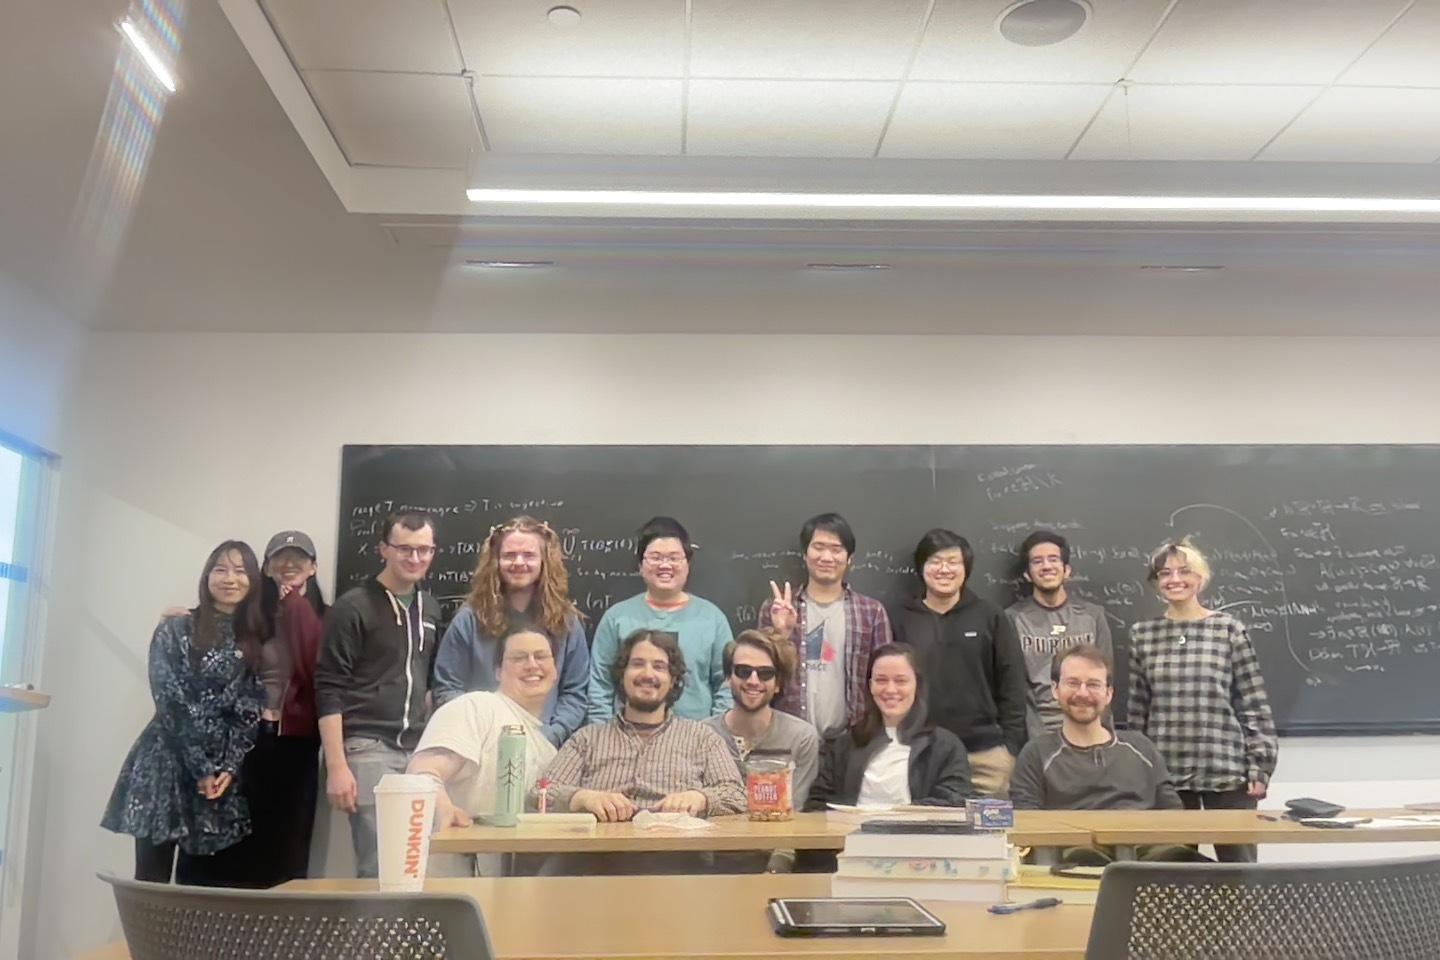
\includegraphics[width=0.5\paperwidth]{FuNtional exam group}
  \end{center}
  
  

\end{thebibliography}

\end{document}